\documentclass{article}

\usepackage{fancyhdr}
\usepackage{extramarks}
\usepackage{amsmath}
\usepackage{amsthm}
\usepackage{amsfonts}
\usepackage{tikz}
\usepackage[plain]{algorithm}
\usepackage{algpseudocode}
\usepackage{enumitem}
\usepackage{listings}

\usetikzlibrary{automata,positioning}


% 
% Python code settings
% 

\lstset{frame=tb,
  language=Python,
  aboveskip=3mm,
  belowskip=3mm,
  showstringspaces=false,
  columns=flexible,
  basicstyle={\small\ttfamily},
  numbers=none,
  numberstyle=\tiny\color{gray},
  keywordstyle=\color{blue},
  commentstyle=\color[rgb]{0.4,0.4,0.4}\ttfamily,
  stringstyle=\color[rgb]{1,0.6,0.2},
  breaklines=true,
  breakatwhitespace=true,
  tabsize=3
}

%
% Basic Document Settings
%

\lstset{%
mathescape=true}

\topmargin=-0.45in
\evensidemargin=0in
\oddsidemargin=0in
\textwidth=6.5in
\textheight=9.0in
\headsep=0.25in

\linespread{1.1}

\pagestyle{fancy}
\lhead{\hmwkAuthorName}
\chead{\hmwkClass\ : \hmwkTitle}
\rhead{\firstxmark}
\lfoot{\lastxmark}
\cfoot{\thepage}

\renewcommand\headrulewidth{0.4pt}
\renewcommand\footrulewidth{0.4pt}

\setlength\parindent{0pt}

%
% Create Problem Sections
%

\newcommand{\enterProblemHeader}[1]{
    \nobreak\extramarks{}{Problem \arabic{#1} continued on next page\ldots}\nobreak{}
    \nobreak\extramarks{Problem \arabic{#1} (continued)}{Problem \arabic{#1} continued on next page\ldots}\nobreak{}
}

\newcommand{\exitProblemHeader}[1]{
    \nobreak\extramarks{Problem \arabic{#1} (continued)}{Problem \arabic{#1} continued on next page\ldots}\nobreak{}
    \stepcounter{#1}
    \nobreak\extramarks{Problem \arabic{#1}}{}\nobreak{}
}

\setcounter{secnumdepth}{0}
\newcounter{partCounter}
\newcounter{homeworkProblemCounter}
\setcounter{homeworkProblemCounter}{1}
\nobreak\extramarks{Problem \arabic{homeworkProblemCounter}}{}\nobreak{}

%
% Homework Problem Environment
%
% This environment takes an optional argument. When given, it will adjust the
% problem counter. This is useful for when the problems given for your
% assignment aren't sequential. See the last 3 problems of this template for an
% example.
%
\newenvironment{homeworkProblem}[1][-1]{
    \ifnum#1>0
        \setcounter{homeworkProblemCounter}{#1}
    \fi
    \section{Problem \arabic{homeworkProblemCounter}}
    \setcounter{partCounter}{1}
    \enterProblemHeader{homeworkProblemCounter}
}{
    \exitProblemHeader{homeworkProblemCounter}
}

%
% Homework Details
%   - Title
%   - Due date
%   - Class
%   - Section/Time
%   - Instructor
%   - Author
%

\newcommand{\hmwkTitle}{Homework\ \#3}
\newcommand{\hmwkDueDate}{September 14, 2018}
\newcommand{\hmwkClass}{COMS 572}
\newcommand{\hmwkClassTime}{}
\newcommand{\hmwkClassInstructor}{Professor Jin Tian}
\newcommand{\hmwkAuthorName}{Le Zhang}

%
% Title Page
%

\title{
    \vspace{2in}
    \textmd{\textbf{\hmwkClass:\ \hmwkTitle}}\\
    \normalsize\vspace{0.1in}\small{\hmwkDueDate\ by 17:00pm}\\
    \vspace{0.1in}\large{\textit{\hmwkClassInstructor\ \hmwkClassTime}}
    \vspace{3in}
}

\author{\textbf{\hmwkAuthorName}}
\date{}

\renewcommand{\part}[1]{\textbf{\large Part \Alph{partCounter}}\stepcounter{partCounter}\\}

%
% Various Helper Commands
%

% Useful for algorithms
\newcommand{\alg}[1]{\textsc{\bfseries \footnotesize #1}}

% For derivatives
\newcommand{\deriv}[1]{\frac{\mathrm{d}}{\mathrm{d}x} (#1)}

% For partial derivatives
\newcommand{\pderiv}[2]{\frac{\partial}{\partial #1} (#2)}

% Integral dx
\newcommand{\dx}{\mathrm{d}x}

% Alias for the Solution section header
\newcommand{\solution}{\textbf{\large Solution}}

% Cartesian product
\newcommand{\Cross}{\mathbin{\tikz [x=1.4ex,y=1.4ex,line width=.2ex] \draw (0,0) -- (1,1) (0,1) -- (1,0);}}%

% Probability commands: Expectation, Variance, Covariance, Bias
\newcommand{\E}{\mathrm{E}}
\newcommand{\Var}{\mathrm{Var}}
\newcommand{\Cov}{\mathrm{Cov}}
\newcommand{\Bias}{\mathrm{Bias}}

\begin{document}

\maketitle

%
% Problem 1
%
\pagebreak
\begin{homeworkProblem}
\textit{(30 pts.)} The \textbf{missionaries and cannibals} problem is usually stated as follows. Three mission- aries and three cannibals are on one side of a river, along with a boat that can hold one or two people. Find a way to get everyone to the other side without ever leaving a group of mis- sionaries in one place outnumbered by the cannibals in that place. This problem is famous in AI because it was the subject of the first paper that approached problem formulation from an analytical viewpoint (Amarel, 1968).



\begin{enumerate}[label=\alph*.]
    \item Formulate the problem precisely, making only those distinctions necessary to ensure a valid solution. Draw a diagram of the complete state space. 
    
    \textbf{Answer:}
    If we use four integers, each from 0 to 3, to represent the number of missionaries and number of cannibals on both sides of the river, we will be able to use four-integer tuples to represent the states. For example, state [2,2,1,1] means there are 2 missionaries and 2 cannibals are on the left side, and 1 missionary and 1 cannibal are on the right side. The state of number of people on boat is not considered as a space state because cannibals can never outnumber missionaries on a boat. 
    \begin{enumerate}
        \item \textbf{Initial State}: 
            All people are on the left side, so we get [3,3,0,0].
        \item \textbf{States}:
            Any combinations of numbers. When missionaries are outnumbered by cannibals on any side, it is a bad state.
        \item \textbf{Actions}:
            Move up to 2 people from one side to the other. We have two directions here, from left to right, and from right to left depending on the position of the boat. We cannot move along one direction twice continuously. For instance, [-2,0,2,0] means that we move 2 missionaries from left side to the right. And the next move should be from right to left.
        \item \textbf{Goal State}:
            All the people are moved to the other side of the river, which is state [0,0,3,3].
    \end{enumerate}
    
    A diagram of complete state space is shown below:
    
    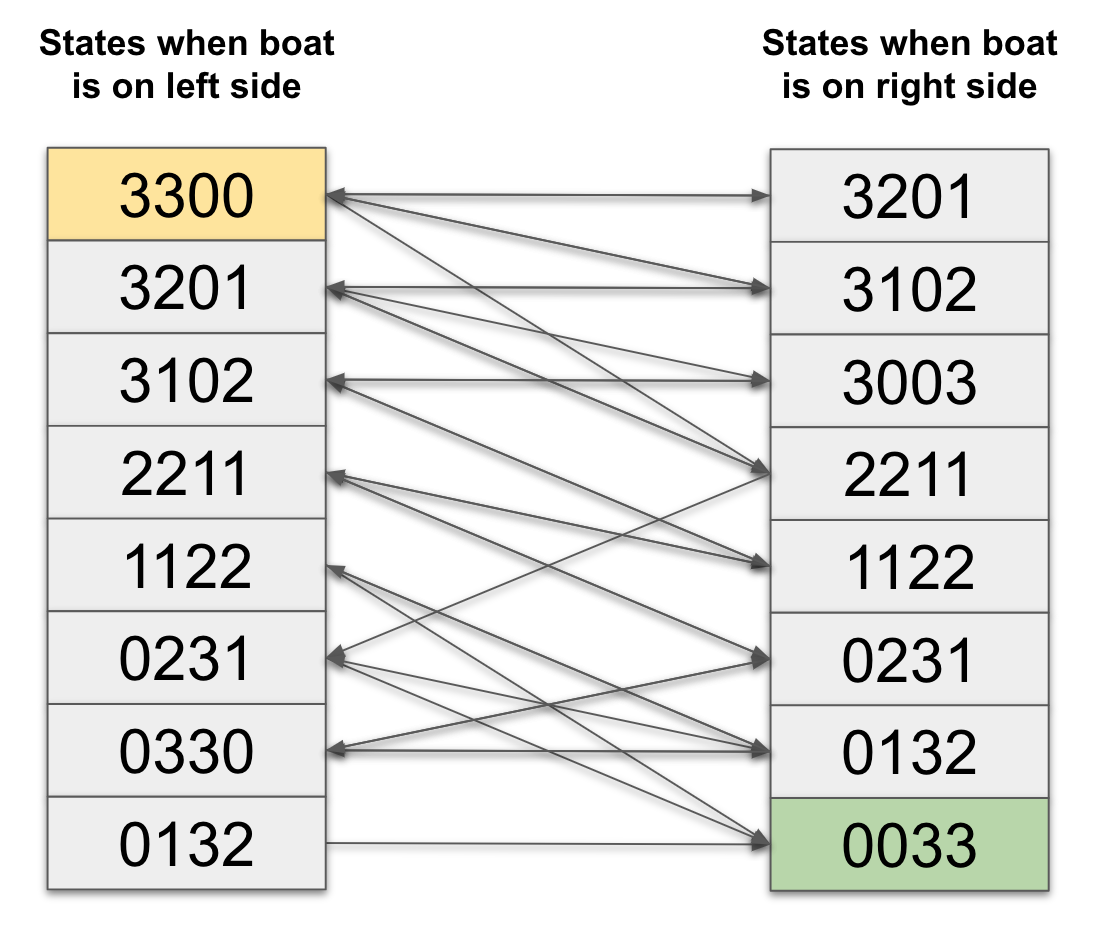
\includegraphics[width=0.8\textwidth]{img/states_diagram.png}
    
    A table of all possible moves and states is shown below:
    
    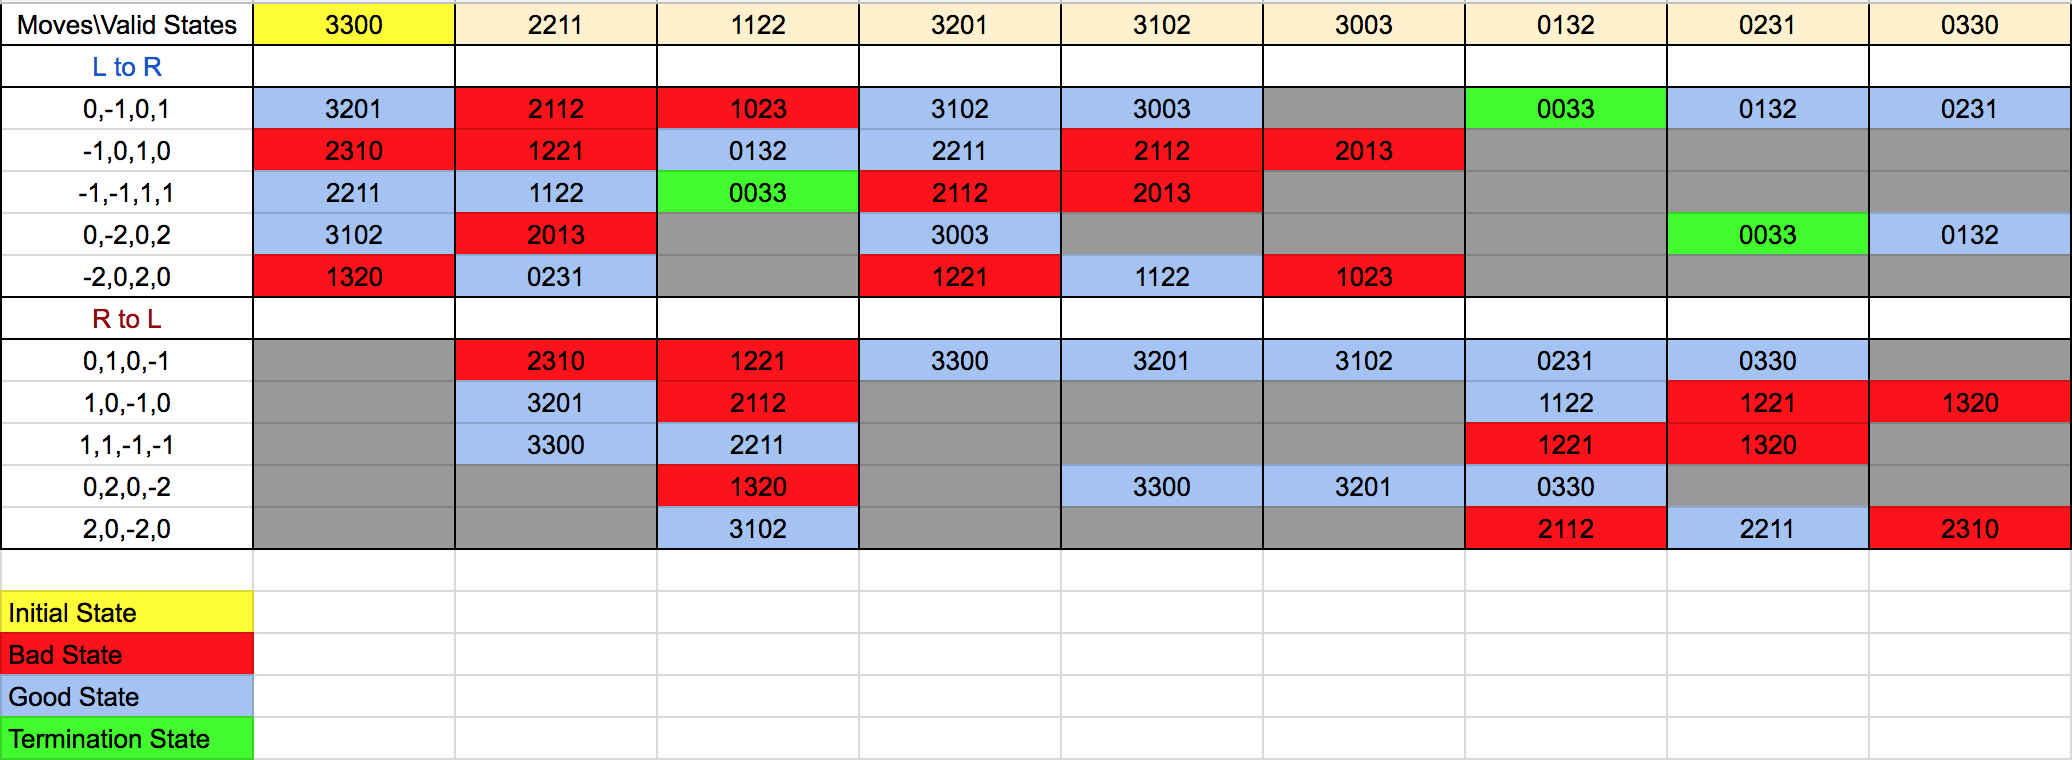
\includegraphics[width=0.92\textwidth]{img/states_table.png}
    
    
    
    
    
    \item Implement and solve the problem optimally using an appropriate search algorithm. Is it a good idea to check for repeated states? 
    
    \textbf{Answer:}
    
    The search algorithm I choose to use is BFS. First, we start from the initial state [3,3,0,0] with boat on the left side. Then, we apply all possible moves from left to right and check if the state after the action is valid. If it is valid, store that state in a list of states for next step. After we go through all the current states, we change the boat position and update the current state list with the list of next states. Then we apply the right to left actions to find out the next possible valid states. Repeat this process until we reach the goal state [0,0,3,3]. 
    
    It is critical to check for repeated states, because you don’t want to get stuck in a loop and waste computing time and memory on those visited paths. It is even more important if we apply DFS because a loop can lead to infinite computing time. 
    
    Down below is a python program I wrote to solve this problem. The source code is attached to the submission. And the solution given by my algorithm is shown below.
    
    \textbf{Solutions:}
    
    \lstinputlisting[language=Python]{mis_can_prob_solution.txt}
    
    \pagebreak
    
    \textbf{Python source code:}
    
    \lstinputlisting[language=Python]{mis_can_prob.py}

    
    \item Why do you think people have a hard time solving this puzzle, given that the state space is so simple?
    
    \textbf{Answer:}
    
    As we can see from the above table, there are 16 possible states on each side, and 10 of them are valid states. If we take the position of boat into consideration, it's 20 possible valid states on both sides. The actions are moving people back and forth on the two sides of a river and the boat position is changing at each step. The searching algorithm for human brain is DFS by default. People feel more comfortable to follow a stream and apply DFS instead of spread out and apply BFS on a specific problem. Unfortunately, DFS is not the best option to this problem because it requires a lot of memory to check repeat states and loops. The 32 possible states and 20 valid states is too much for human being to apply BFS with. Therefore, this problem seems to be easy for computers but hard for human. 

\end{enumerate}

\end{homeworkProblem}

\pagebreak
\begin{homeworkProblem}
\textit{(20 pts.)} Consider a state space where the start state is number $1$ and each state $k$ has two successors: numbers $2k$ and $2k + 1$.

\begin{enumerate}[label=\alph*.]
    \item Draw the portion of the state space for states 1 to 15.
    
    \textbf{Answer:}
    
    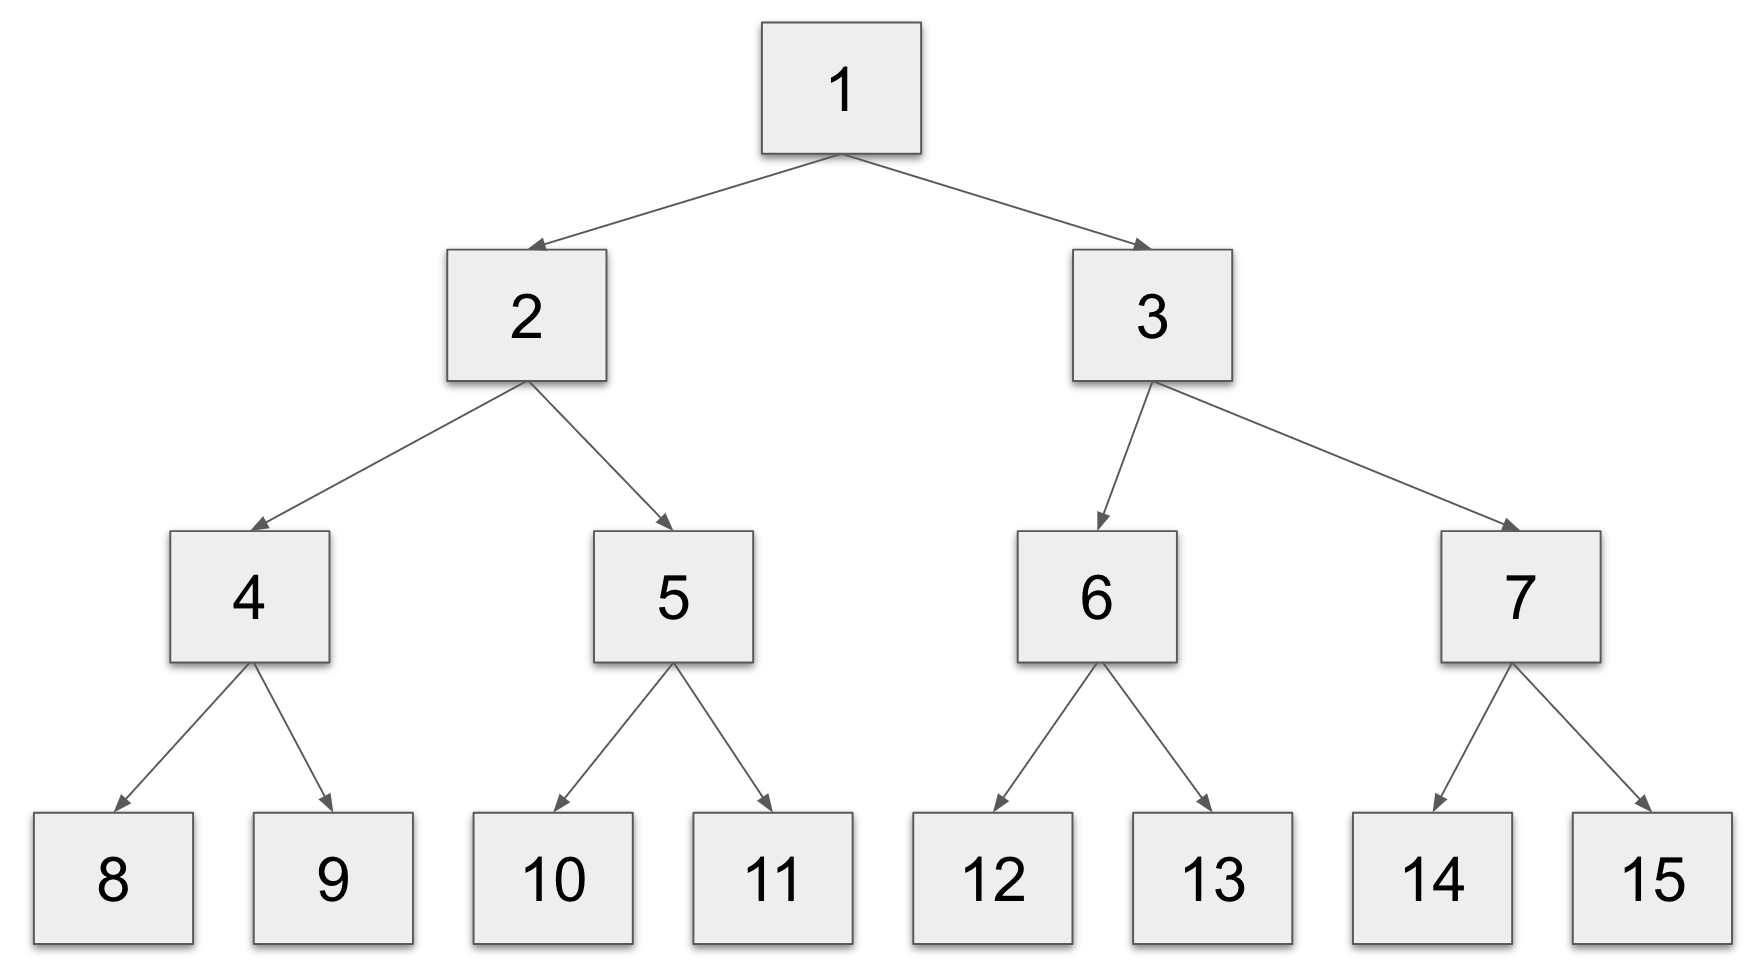
\includegraphics[width=0.8\textwidth]{img/p2_1.png}
    
    \item Suppose the goal state is 11. List the order in which nodes will be visited for breadth-first search, depth-limited search with limit 3, and iterative deepening search.

    \textbf{Answer:}
    
    \textbf{BFS:}
    
    $1\xrightarrow{}2\xrightarrow{}3\xrightarrow{}4\xrightarrow{}5\xrightarrow{}6\xrightarrow{}7\xrightarrow{}8\xrightarrow{}9\xrightarrow{}10\xrightarrow{}11$
    
    \textbf{DLS:}
    
    $1\xrightarrow{}2\xrightarrow{}4\xrightarrow{}8\xrightarrow{}9\xrightarrow{}5\xrightarrow{}10\xrightarrow{}11$
    
    \textbf{IDS:}
    
    \begin{enumerate}
    
    \item[$\square$] Iter\_1 Depth 0:
    
    $1$
    
    \item[$\square$] Iter\_2 Depth 1:
    
    $1\xrightarrow{} 2\xrightarrow{} 3$
    
    \item[$\square$] Iter\_3 Depth 2:
    
    $1\xrightarrow{} 2\xrightarrow{} 4\xrightarrow{} 5\xrightarrow{} 3\xrightarrow{} 6\xrightarrow{} 7$
    
    \item[$\square$] Iter\_4 Depth 3:
    
    $1\xrightarrow{} 2\xrightarrow{} 4\xrightarrow{} 8\xrightarrow{} 9\xrightarrow{} 5\xrightarrow{} 10\xrightarrow{} 11$
    
    \end{enumerate}
    

\end{enumerate}

\end{homeworkProblem}

% \pagebreak
% \begin{thebibliography}{9}
% \bibitem{AI_textbook} 
% Russell, Stuart and Norvig, Peter. 
% \textit{Artificial Intelligence: A Modern Approach}. 
% Prentice Hall Press, Upper Saddle River, NJ, USA, 2009.
 
% \bibitem{wiki_Loebner} 
% \texttt{https://en.wikipedia.org/wiki/Loebner\_Prize}

% \bibitem{wiki_Turing_test} 
% \texttt{https://en.wikipedia.org/wiki/Turing\_test}

% \bibitem{wiki_Mitsuku} 
% \texttt{https://en.wikipedia.org/wiki/Mitsuku}
 
% \bibitem{loabner_prize} 
% \texttt{https://www.aisb.org.uk/events/loebner-prize}

% \bibitem{LP2017}
% \texttt{https://chatbotsmagazine.com/how-to-win-a-turing-test-the-loebner-prize-3ac2752250f1}

% \bibitem{alphagozero}
% Silver, David, et al.
% \textit{Mastering the game of Go without human knowledge}. 
% Nature, Macmillan Publishers Limited, 2017.

% \bibitem{mitsuku}
% \texttt{https://www.pandorabots.com/mitsuku/}

% \end{thebibliography}

\end{document}
